%%%%%%%%%%%%%%%%%%%%%%%%%%%%%%%%%%%%%%%%%
% UMPU
%%%%%%%%%%%%%%%%%%%%%%%%%%%%%%%%%%%%%%%%%
\section{Micro Memory Protection Unit}
\label{sec:umpu}
%
A completely software-based approach to memory protection incurs a
large performance penalty despite the performance optimizations.
%(Section~\ref{sec:bitmasklut}).
%
A detailed discussion of the overheads can be found in
Section~\ref{sec:eval}.
%
The additional CPU cycles introduced due to the run-time checks in
Harbor may not be tolerable in certain performance sensitive
applications such as Vango~\cite{ben06vango}.
%
In this section, we extend the ideas of Harbor memory protection to
design a memory protection unit for embedded processors like those
%
%Tiny embedded processors refers to the severely resource constrained
%8-bit and 16-bit microcontrollers 
commonly found in mote class sensor nodes
%
%Examples of such microcontrollers are 
such as Atmel's ATMEGA128L~\cite{avrdatasheet} or TI's
MSP430~\cite{mspdatasheet}.
%
We call the result a \emph{micro memory protection unit}, or UMPU.
%
%We present Micro Memory Protection Unit (UMPU) that is designed for
%resource constrained tiny embedded processors.
%
Our approach is motivated by the fault isolation principles of Harbor
and is fundamentally different from memory protection units found in
some of the higher-end embedded processors (Section~\ref{sec:mpu}).
%
We do not partition the address space of the microcontroller.
%
%Available memory on microcontrollers is severely limited.
%
%For example, ATMEGA128 AVR has only 4 KB of on-chip RAM.
%
%In most systems~\cite{hill02micro}, this is the total available memory.
%
%Static partitioning would further limit the memory that is available
%to individual software components.
%
Instead we rely on Harbor's Memory Map data structure to efficiently
record ownership and layout information of the entire address space.
%

The key difference between UMPU and any software-based fault isolation
system is that UMPU does not rewrite the binary to introduce run-time
checks.
%
UMPU instead enhances the implementation of \texttt{store, call} and
\texttt{return} instructions in the microcontroller to perform
run-time checks in hardware.
%
This minimizes the performance overhead of performing run-time checks
in software and also eliminates the binary rewrite step of SFI.

\begin{figure}[htbp]
   \centering
   \includegraphics[height = 2.0in,
   keepaspectratio=true]{figures/umpuoverview.eps} 
   \caption{UMPU Overview}
   \label{fig:umpuoverview}
\end{figure}
%
UMPU can be viewed as a hardware/software co-design approach to memory
protection (Figure~\ref{fig:umpuoverview}).
%
Low cost architecture extensions and a software run-time library work
together to isolate different software components running on an
embedded processor.
%
%UMPU can be implemented entirely in software (as shown already)
%albeit a performance overhead.
%
Simple enhancements to the microcontroller core enable us to perform
critical operations in hardware, thereby improving Harbor's
performance significantly.
%
%-----------------------------------------------------------
\subsection{UMPU Overview}
%
An overview of our system highlighting all its components is shown in
Figure~\ref{fig:umpuoverview}.
%
The final firmware image is composed of multiple software modules that
need to be protected from one another.
%
%The software components are installed in separate protection domains.
%
A cross domain linking mechanism described in
Section~\ref{sec:cross_domain_linking} installs the software modules
in separate protection domains.
%
%The cross domain linker generates 
A software jump table assists the domain tracker within the processor
in determining the identity of the currently active domain.
%
The \emph{Control flow controller} (Section~\ref{sec:cfctrl}) ensures control flow integrity through a cross domain call unit and a domain bounds checker.
%
A safe stack located in protected memory stores UMPU state information during cross domain calls.
%
The memory map tracks layout and ownership information for the protected address space.
%
The firmware image running on the processor, checked by the  memory
map controller (Section~\ref{sec:mmc}) is guaranteed to be memory
safe.
%
%The safe stack stores the return addresses in protected memory and 
%ensures control flow integrity within a module.
%

Upon reset, the processor boots into the trusted domain.
%
The code executing in the trusted domain is not subject to any checks.
%
The software library in the trusted domain configures UMPU by
initializing the configuration registers.
%
It also initializes the memory map.
%
The UMPU configuration registers are made read only when the control
flow leaves the trusted domain, thereby avoiding any chance of
corruption.
%
The protection is enabled by setting the \texttt{UMPU\_EN} bit in the
\texttt{umpu\_config} register.
%
%
%-----------------------------------------------------------
\subsection{Memory Map Controller}
\label{sec:mmc}
%
The memory map controller (MMC) is a functional unit that interacts with
the memory map to validate memory accesses made by software
components.
%
It enforces the protection model that we described earlier; programs
can write only into their domain.
%
The MMC intercepts the signals generated by the CPU for writing into
data memory (Figure~\ref{fig:mmcramcpu}).
%
If the write address is valid, then the MMC writes directly into data
memory.
%
\begin{figure}[htbp]
   \centering
   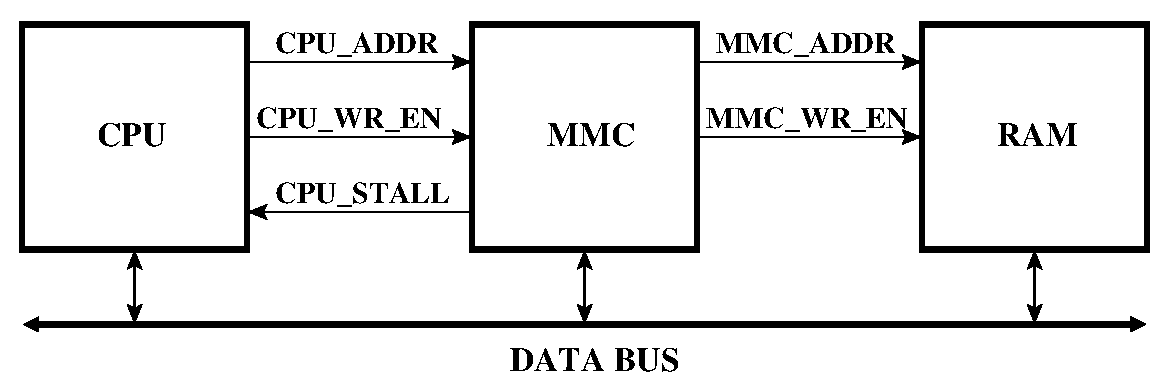
\includegraphics[height=1in,
   keepaspectratio=true]{figures/mmcramcpu.eps} 
   \caption{Memory Map Controller (MMC)}
   \label{fig:mmcramcpu}
\end{figure}
%
\begin{figure}[htpb]
 \centering
  \mbox{
    \subfigure[Regular Store]{\label{fig:mmcopst}\includegraphics[width=2.5in,
      keepaspectratio = true]{figures/mmcop_st.eps}}
    \hspace{0.2in}
    \subfigure[Safe Store]{\label{fig:mmcopsafest}\includegraphics[width=2.5in,
      keepaspectratio = true]{figures/mmcop_safe_st.eps}}
  }
  \caption{MMC Timing Diagram}
\end{figure}   
% %
% \begin{figure}[htbp]
%    \centering
%    \includegraphics[height=2in,
%    keepaspectratio=true]{figures/mmcop.eps} 
%    \caption{Memory Map Controller (MMC)}
%    \label{fig:mmcop}
% \end{figure}
% %z
%-----------------------------------------------------------------
\subsubsection{MMC Operation}
%
We describe the MMC's operation of MMC by explaining the steps in
the execution of a store instruction.
%
Regular store operation takes two clock cycles on AVR.
%
In the first clock cycle, the instruction is decoded and the data to
be written is read from the register file.
%
The processor issues the write address and the write enable in the
second clock cycle.
%
This is illustrated in Figure~\ref{fig:mmcopst}.
%
In the protected mode, the store operation requires an additional
clock cycle (Figure~\ref{fig:mmcopsafest}).
%
The operation in the first clock cycle is similar to a regular store:
instruction decoding followed by a read of the data to be written from
the register file.
%
In the subsequent clock cycles, the MMC performs three operations.
%
First, it stalls the processor execution and takes control of the
address bus to memory.
%
This occurs in the second cycle.
%Figure~\ref{fig:mmcopsafest}.
%
In the same clock cycle it performs an address translation operation
to determine the address of the permissions in the memory map.
%
Address translation is implemented as combinational logic, as shown in
Figure~\ref{fig:umpuaddrtans}.
%
Memory map permissions are also read in this cycle as the MMC unit has
control over the address bus.
%
Second, the MMC compares the ownership information to the identity of
the current executing domain.
%
The combinational logic of the checker is shown in
Figure~\ref{fig:umpupermscheck}.
%
Finally, if the check is successful, then the MMC issues a write
enable signal to the data memory; else an \texttt{MMC\_PANIC} signal is
asserted.
%
%
\begin{figure}[htpb]
 \centering
  \mbox{
    \subfigure[Address
    Translation]{\label{fig:umpuaddrtans}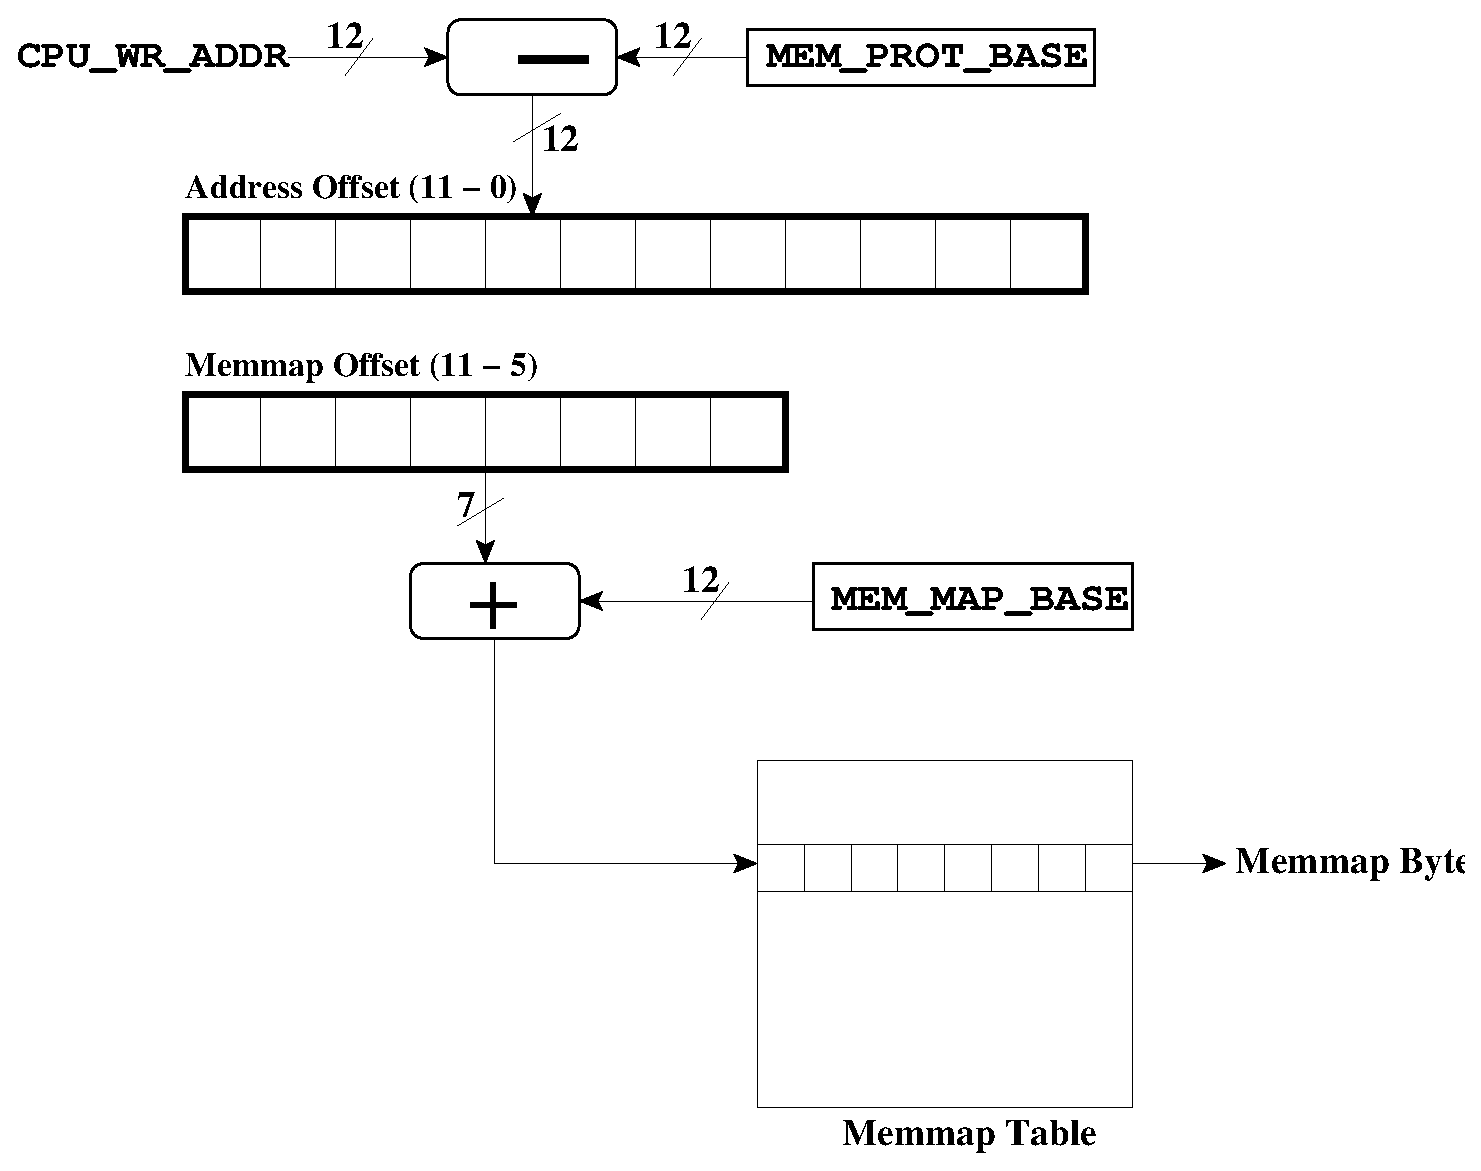
\includegraphics[width=2.5in,
      keepaspectratio = true]{figures/umpuaddrtans.eps}}
    \hspace{0.2in}
    \subfigure[Permission
    Checker]{\label{fig:umpupermscheck}\includegraphics[width=2.5in,
      keepaspectratio = true]{figures/umpupermscheck.eps}}
  }
  \caption{MMC Operations (8-domain)}
\end{figure}   
%
%
%----------------------------------------------
\subsubsection{MMC Software Library}
\label{sec:mmc_for_protection}
%
The software library is responsible for the initialization of the MMC.
%
The memory map controller is configurable through a set of
programmable registers shown in Table~\ref{tab:mmap_config_regs}.
%
The registers are accessible only from the trusted domain.
%
The address range to be protected by the memory map is input to the
software library; the library appropriately initializes the registers
\texttt{mem\_prot\_base} and \texttt{mem\_prot\_top}.
%
It provides macros to initialize the \texttt{mem\_map\_config}
register, which configures the block size and the number of protection
domains available in the system.
%
Our design is flexible to accommodate different block sizes and number
of domains.
%
\begin{table}[htdp]
\centering
\small{
\begin{tabular}{|l|l|}
	\hline
	Register & Function\\
	\hline
	\texttt{mem\_map\_base} & Memory map base pointer \\
	\texttt{mem\_prot\_base} & Lower bound of protected address space\\
	\texttt{mem\_prot\_top} & Upper bound of protected address space\\
	\texttt{mem\_map\_config} & Configure block size and domains\\
	\hline
\end{tabular}}
\caption{Memory Map Configuration Registers}
\label{tab:mmap_config_regs}
\end{table}

The software library also manages the memory map.
%
It provides custom implementations of the \texttt{malloc},
\texttt{free} and \texttt{change\_own} calls, as described.
% that are carefully designed to protect against some common
% programming bugs discussed in Section~\ref{sec:mmap_for_protection}.
%
A special read-only register contains the identity of the currently
execution domain.
%
This register is tracked and updated by the domain
tracker (Section~\ref{sec:domtracker}).
%
All the APIs in the software library only trust the information stored
in this register.
%
For example, the memory map is updated with the identity stored in
this register during a call to \texttt{malloc}.
%
%------------------------------------------------------------
\subsection{Control Flow Controller}
\label{sec:cfctrl}
%
The control flow controller (CFC) ensures that control can never flow out of
a domain, except via calls to functions exported by other domains, and
via returns to calls from other domains.
%
Conversely, control flow can enter a domain only through an exported
function or through the return site of a call that is made to a
function exported by some other domain.
%
%In this section, we describe the different functional units that constitute the Control Flow controller.
%
The CFC comprises software run-time components, desktop tools, and
hardware functional units that work together to ensure control flow
integrity.
%
The cross domain linker (Section~\ref{sec:cross_domain_linking}) sets up the domains and the jump table in the program memory.
%
The cross domain call unit (Section~\ref{sec:cdcunit}) implements the
cross domain call mechanism using the domain tracker
(Section~\ref{sec:domtracker}) and a safe stack
(Section~\ref{sec:umpuss}).
%
The domain bounds checker (Section~\ref{sec:dombndschecker}) ensures
that the control flow never leaves a domain except through valid
points.
%
This section describes all the components of CFC.
%This section describes the design of CFC components and the linking mechanism used to implement cross domain calls.
%---------------------------------------------------
\subsubsection{Cross Domain Linking}
\label{sec:cross_domain_linking}
%
Cross domain linking is a mechanism by which the function calls frome
one domain to another are linked through a jump table,
%
as described in Section~\ref{sec:crossdomcall}.
%
%is similar in design to the processor interrupt vector table.
%
%Each entry in jump table is an instruction to jump to a valid
%exported function.
%
% Each domain has its own jump table that contains all functions that
% it exports. 


%The set of functions exported by a domain are parsed by a cross domain
%linker tool that automatically generates a jump table in the
%flash memory.
%
In the current implementation, the jump table is generated manually
and cross domain functions are invoked through wrappers that
call into the jump table.
%
This process can be automated if the programming language
contains semantics that define an interface for a module (for
e.g. NesC) or the system has provision for explicitly recording an interface
(e.g. a module header in SOS).
%The current implementation of the cross domain linker simply parses a
%header file that contains all the functions exported by a domain.
%
%It then generates a jump table using the symbol names of the exported
%functions.
%
%All the references to the exported functions are replaced by references to
%the corresponding entries in the jump table.
%
%The linker can be improved if the programming language contains
%semantics that define an interface.
%
%An example of such a language that is popular in sensor networks is
%NesC~\cite{gay03nesc}.
%-----------------------------------------------------------
\subsubsection{Cross Domain Call Unit}
\label{sec:cdcunit}
%
This section describes the design and implementation of the cross domain call unit in UMPU.
%
The operations performed during the cross domain call are similar to
the Harbor's cross domain call described in
Section~\ref{sec:crossdomcall}.
%

A cross domain call is triggered whenever the control flow reaches the
jump table through any of the call instructions.
%
As shown in Figure~\ref{fig:cdcinit}, the base address of the jump
table is stored in the UMPU register
\texttt{umpu\_jmp\_tbl\_base\_ptr}.
%
This register is initialized during boot up by the software library.
%
The signals indicating a call instruction and the call address are
provided by the fetch decoder unit in the processor.
%
The combinational logic in the cross domain call unit asserts the \texttt{UMPU\_CDC\_EN} signal.
%
This signal triggers the cross domain call state machine as shown in Figure~\ref{fig:cdcstmc}.
%
The state machine pushes the previous domain ID, stack bounds and cross domain return address onto the safe stack.
%
The new domain ID is updated by the domain tracker.
%
The new stack bounds is determined from the run-time stack pointer.
%
The new cross domain return address is updated by the fetch decoder unit.
%
\begin{figure}[htpb]
 \centering
  \mbox{
    \subfigure[Cross Domain Call Init]{\label{fig:cdcinit}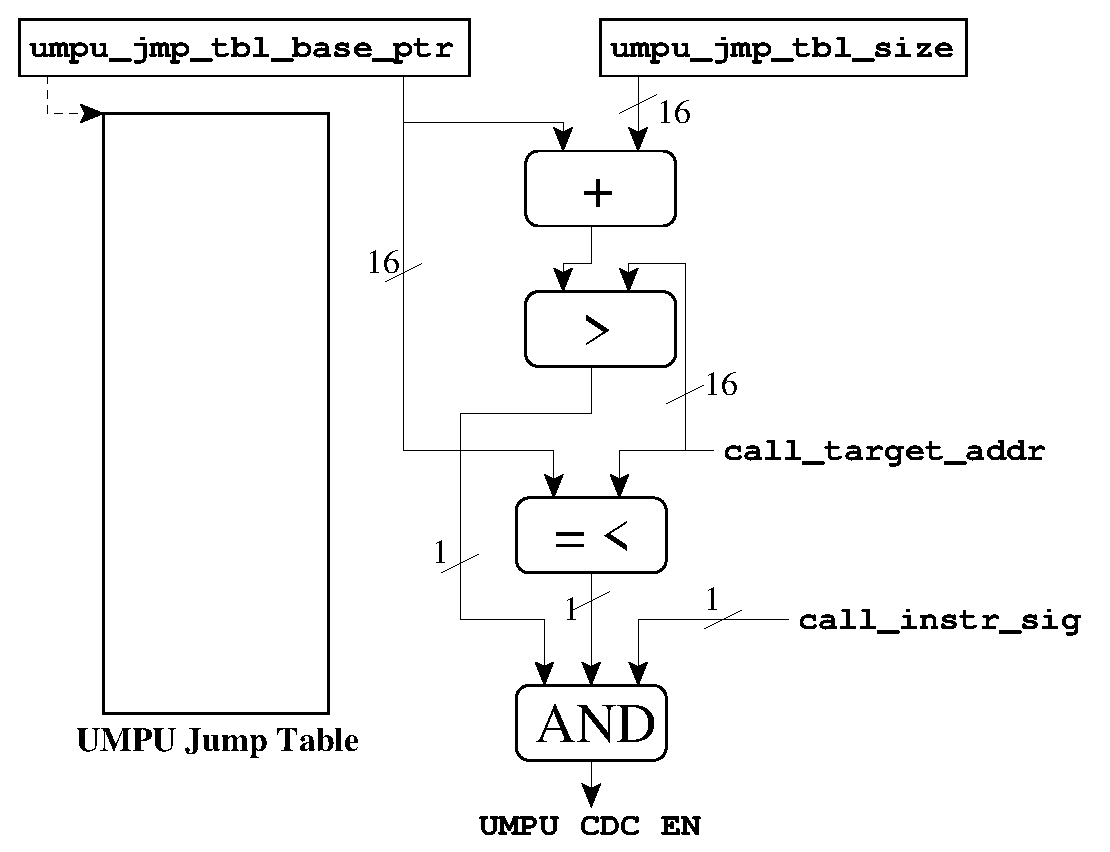
\includegraphics[width=2.5in,
      keepaspectratio = true]{figures/umpucdcinit.eps}}
    \hspace{0.2in}
    \subfigure[Cross Domain Call State Machine]{\label{fig:cdcstmc}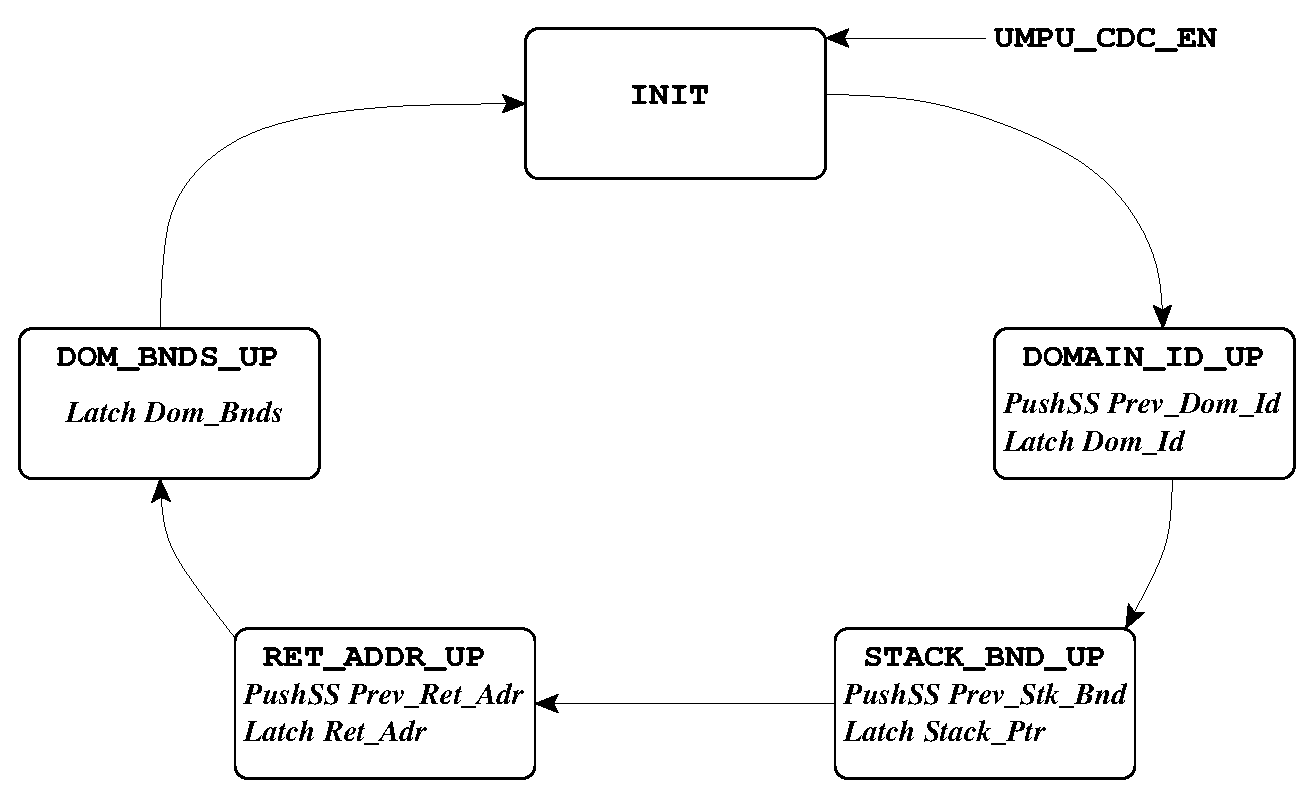
\includegraphics[width=2.5in,
      keepaspectratio = true]{figures/cdcstatemc.eps}}
  }
  \caption{Cross Domain Call Unit}
\end{figure}   

A cross domain return is triggered during the execution of a processor's \texttt{ret} instruction.
%
The signals indicating a \texttt{ret} instruction and the return address are sent to the cross domain call unit by the processor's fetch decoder unit.
%
A cross domain return is initiated if the return address matches the stored cross domain return address.
%
During a cross domain return, the previous values of the domain ID, stack bounds and cross domain return address are restored from the safe stack.
%
The cross domain return is also implemented as a state machine.
%
%---------------------------------------------------
\subsubsection{Domain Tracker}
\label{sec:domtracker}
%
The domain tracker is a functional unit that tracks the execution of
the currently executing domain.
%
The updated domain ID is stored in a special read-only register.
%
The value stored in the register is used by the memory map controller
to validate the access permissions for a store operation.
%
The domain tracker is triggered by the \texttt{UMPU\_CDC\_EN} signal
(Figure~\ref{fig:cdcinit}) or by the occurrence of an interrupt.
%
We discuss interrupts later in Section~\ref{sec:umpuintr}.
%
The jump tables of all the domains are located next to one another in
the program memory.
%
The maximum number of entries in the jump table for a domain is
configured in the \texttt{umpu\_dom\_jmp\_tbl\_size}.
%
Once triggered, the functional unit subtracts the
\texttt{umpu\_jmp\_tbl\_base\_ptr} from the cross domain call address
to determine the offset into the jump table.
%
The offset is divided by the size of a domain's jump table to
determine the new domain ID.
%
The combinational logic implementing the domain tracker is shown in
Figure~\ref{fig:domtracker}.
%
The number of entries is chosen to be a power of 2 to implement the
division operation as a shifter.
%
 \begin{figure}[htbp]
    \centering
    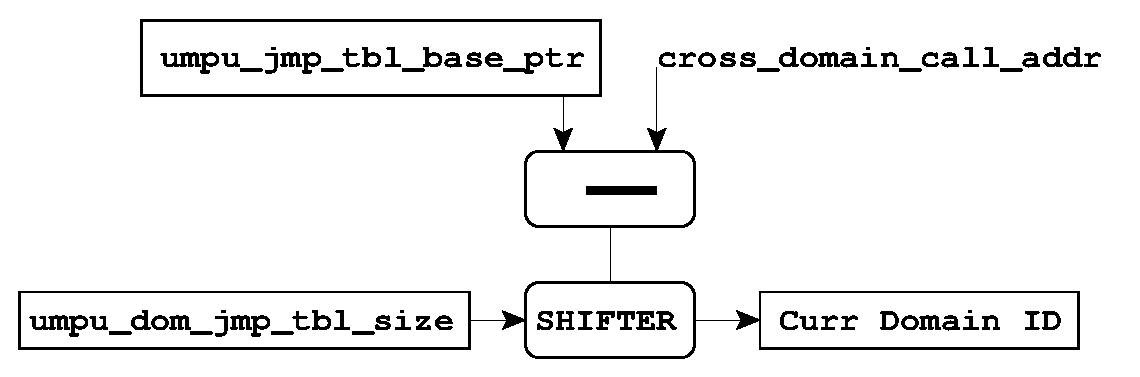
\includegraphics[height=1in,
    keepaspectratio=true]{figures/domtracker.eps} 
    \caption{Domain Tracker}
    \label{fig:domtracker}
 \end{figure}

%---------------------------------------------------
\subsubsection{Safe Stack}
\label{sec:umpuss}
%
UMPU maintains a separate stack in the protected region of memory to
store important state information related to cross domain calls
(Figure~\ref{fig:cdcstmc}).
%
The \texttt{safe\_stack\_ptr} is initialized by the software library
to reside in a protected region of data memory.
%
The hardware does not check whether the safe stack is protected or not.
%
The size of the safe stack is set during initialization.
%
The hardware checks to ensure that safe stack does not overflow.
%
%-----------------------------------------------------------
\subsubsection{Domain Bounds Checker}
\label{sec:dombndschecker}
%
The domain bounds checker ensures that the control flow does not leave
a domain except through the jump table.
%
The program memory layout showing different domains, jump table,
interrupt table and the bootloader is shown in
Figure~\ref{fig:progmemlayout}.
%
The program memory address space can be statically partitioned
or it can use a mechanism similar to the SOS module
loader~\cite{ram05sos}.
%
But the end result of either mechanism is that there is no overlap in
the address space of any modules.
%
Based on this assumption, the domain bounds checker comprises two
components (Figure~\ref{fig:dombndscheck}).
%
First, a \emph{domain bounds table} stores the lower and upper
address bounds for every domain.
%
Second, a \emph{PC bounds checker}, implemented as a combinational
logic block, ensures that the program counter always lies within the
bounds of the current domain or in the jump table.
%
\begin{figure}[htbp]
   \centering
   \includegraphics[height=1in,
   keepaspectratio=true]{figures/progmemlayout.eps} 
   \caption{Program Memory Layout}
   \label{fig:progmemlayout}
\end{figure}
\begin{figure}[htbp]
   \centering
   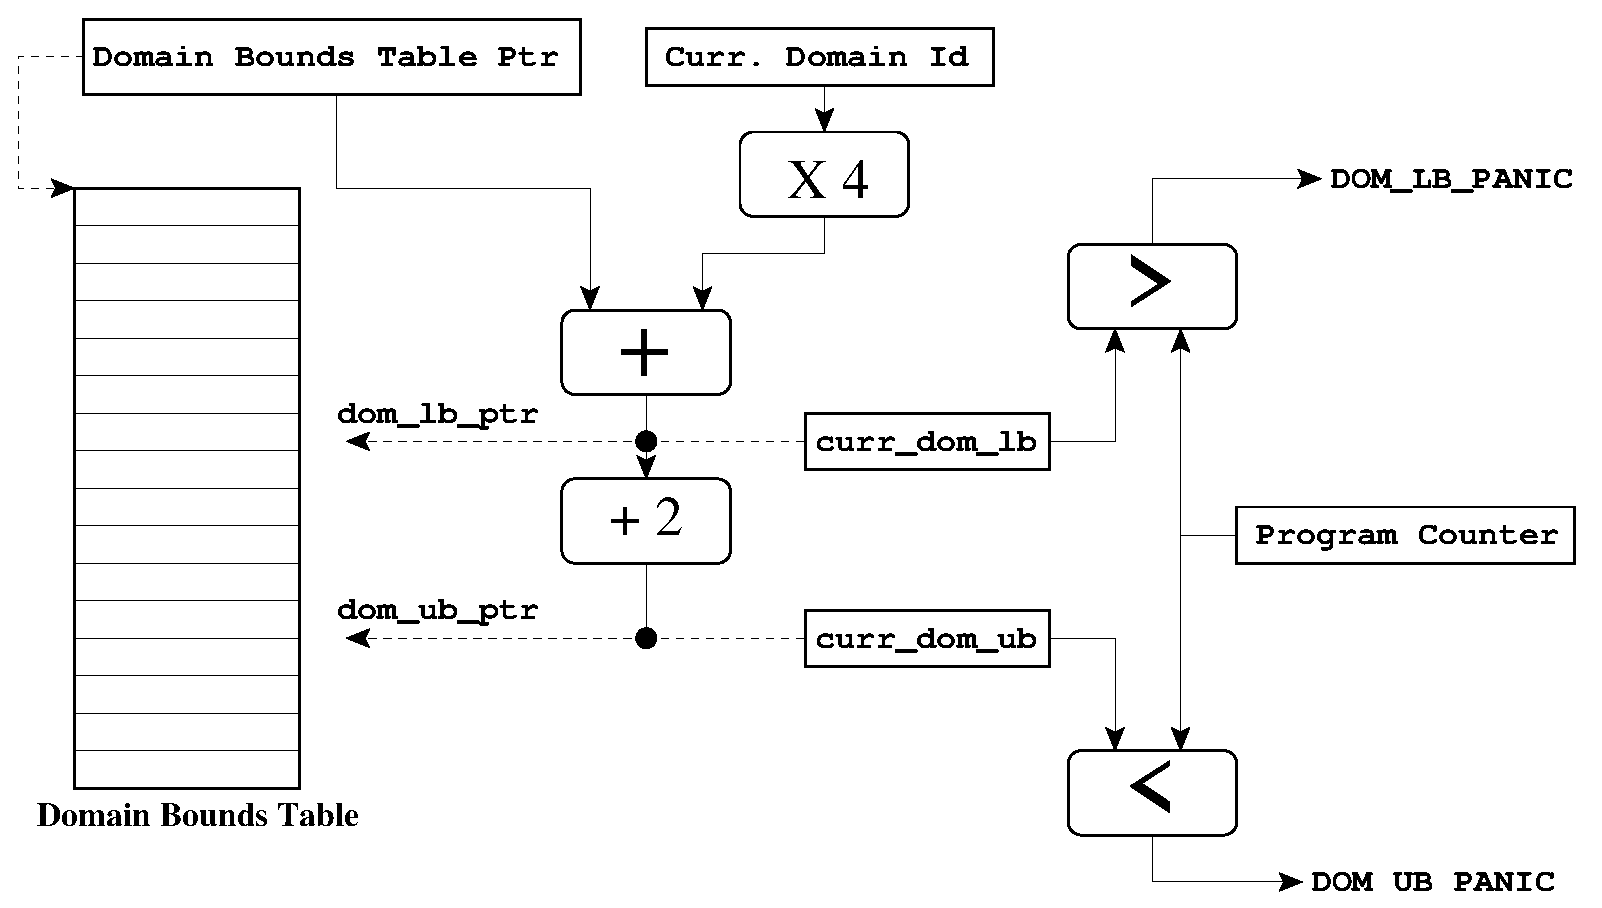
\includegraphics[height=2.5in,
   keepaspectratio=true]{figures/domboundschecker.eps} 
   \caption{Domain Bounds Checker (8 Domains)}
   \label{fig:dombndscheck}
\end{figure}

The domain bounds table can be statically initialized or it
can be filled by a module loader running in the trusted domain.
%
As shown in Figure~\ref{fig:dombndscheck}, the registers
\texttt{dom\_lb\_bnd} and \texttt{dom\_ub\_bnd} store the lower and the
upper bounds of the addresses for the current domain.
%
These registers are updated during every cross domain call.
%
There are two alternate implementations of the domain bounds checker
that have a different performance and area utilization.
%
The domain bounds table can be implemented as a RAM/FLASH based
look-up table or it can be implemented as a register array.
%
The look-up table has more overhead than a register array
implementation because the bounds values for a domain have to be
loaded from memory onto the registers; the bounds can be directly read
from a register array.
%
The register array occupies more area and therefore increases the area
of the processor.
%
We have opted for the register array implementation as it improves the
performance of the system.
%
The PC bounds checker issues a panic signal when the program counter
lies outside the domain bounds.
%
The panic signal is suppressed if the new program counter lies within
the jump table or the interrupt vector table.
%
%------------------------------------------------------------
\subsection{Run-Time Stack Integrity}
\label{sec:umpuruntimestackprot}
%------------------------------------------------
\subsubsection{Stack Bounds Protection}
The run-time stack is protected from cross domain corruption through
the usage of stack bounds.
%
The stack bounds are set by storing the value of the stack pointer
during a cross domain call.
%
The functional unit performs two checks.
%
The first check is an extension to the memory map controller shown in
Figure~\ref{fig:stackbndscheck}.
%
All store instructions whose address is greater than the current stack
bound and lesser than the run-time stack base address are invalid.
%
An \texttt{MMC\_STACK\_PANIC} signal is generated upon an invalid stack
access.
%
The \texttt{stack\_base} register is set to the initial value
of the stack pointer during bootup.
%
The base register is required to allow the stack pointer to be setup
anywhere in the data memory.
%
The second check is to protect against stack underflow within a domain
that could occur due to mismatched push and pops.
%
A \texttt{STACK\_UNDERFLOW\_PANIC} is generated upon error.
%
\begin{figure}[htbp]
  \centering
  \includegraphics[height=1in,
  keepaspectratio=true]{figures/umpustackprot.eps} 
  \caption{Run-Time Stack Checker}
  \label{fig:stackbndscheck}
\end{figure}
%
%--------------------------------------------
\subsubsection{Stack Overflow Protection}
A simple stack overflow check is also implemented that
triggers a panic when the stack pointer exceeds a pre-initialized
upper bound.
%-------------------------------------------
\subsubsection{Return Address Protection}
%
Stack bounds protection cannot prevent stack corruption internal to the domain.
%
Such corruption can modify the return addresses stored on the run-time stack.
%
The domain bounds checker will detect such corruption if the return address lies outside the domain bounds;
%
however, control flow integrity within the domain is not preserved as
the return address could be any arbitrary value within the bounds of
the domain.
%
UMPU preserves control flow integrity within a domain by copying the
return address to the safe stack in the implementation of the call
instruction.
%
Correspondingly, the implementation of the return instruction is also
modified to use the return address present in the safe stack.
%
Return address protection increases the run-time size of the safe stack.
%
%------------------------------------------------------------
\subsection{Interrupt Handler Unit}
\label{sec:umpuintr}
%
The processor's interrupt handling is modified to incorporate memory
protection extensions.
%
In UMPU, by default, all the interrupts are handled in the trusted domain.
%
A verifier running on the desktop scans the interrupt vector table to
ensure that no interrupt handler is located outside the trusted
domain.
%
When the processor begins handling a pending interrupt, it generates a
signal that triggers the UMPU interrupt handler unit.
%
The processor is stalled for a single clock cycle by the interrupt
handler unit while the domain tracker is signaled to update the current
domain ID to the trusted domain.
%
The previous domain ID is pushed onto the safe stack.
%
Thereafter, the control flow within the interrupt handler proceeds as
normal.
%
There are no checks during the execution of the handler in the trusted
domain.
%
But cross domain calls in the interrupt handler can transfer control
to the other domains.
%
Therefore, any domain can process the interrupt despite its origin in
the trusted domain.
%

All processors have a special \texttt{reti} instruction to return from
the interrupt and resume normal execution.
%
UMPU modifies the implementation of \texttt{reti} to include an extra
clock cycle to restore the domain ID of the interrupted domain from
the safe stack.
%
In addition, UMPU disallows the execution of the \texttt{reti} instruction from the non-trusted domain.

An alternate design is to register an interrupt with any
domain.
%
The registration information is stored along with the interrupt
vector table.
%
This allows the processor to directly transfer control to the registered domain
upon receiving an interrupt.
%
This design will have a lower overhead but will incur the cost of a
registration table in FLASH/RAM.
%------------------------------------------------------------
\subsection{UMPU Exception Controller}
%
We implemented an exception mechanism in UMPU to allow the
embedded software to perform suitable recovery in the event of a panic
condition.
%
The UMPU exception controller monitors all the panic signals that can
be generated by the various UMPU extensions.
%
Whenever any panic signal goes high, it generates an interrupt
condition.
%
The interrupt is set to have the highest priority.
%
Further, the interrupt is set to be non-maskable that guarantees its
delivery under all conditions.
%
The Controller also stores some information relating to the exception
that enables the design of recovery routines.
%
For example, the Controller stores the cause of the exception, the
program counter at which the exception occurs and the stack pointer.
%
Table~\ref{tab:umpuexceptions} contains the UMPU exception signals and
the conditions that trigger them.
%
\begin{table}[htdp]
\centering
\small{
\begin{tabular}{|l|l|}
	\hline
	Signal & Condition\\
	\hline
	\texttt{MMC\_PANIC} & Memory map permission violation
        (Fig.~\ref{fig:umpupermscheck})\\
	\texttt{MMC\_STACK\_PANIC} & Run-time stack bounds violation
        (Fig.~\ref{fig:stackbndscheck})\\
	\texttt{STACK\_UNDERFLOW\_PANIC} & Stack pointer lower than
        the stack bound (Fig.~\ref{fig:stackbndscheck}) \\
	\texttt{STACK\_OVERFLOW\_PANIC} & Stack overflow violation
        (Sec.~\ref{sec:umpuruntimestackprot})\\
        \texttt{DOM\_LB\_PANIC} & Control flow outside domain lower
        bound (Fig.~\ref{fig:dombndscheck})\\
        \texttt{DOM\_UB\_PANIC} & Control flow outside domain upper
        bound (Fig.~\ref{fig:dombndscheck})\\
	\hline
\end{tabular}}
\caption{UMPU Exception Signals and Conditions}
\label{tab:umpuexceptions}
\end{table}

%------------------------------------------------------------
\subsection{Configurable Soft-Core}
%
The UMPU extensions are
%have been designed with a lot of flexibility that enables them to be 
configurable by software at run-time.
%
For example, the block size used in the memory map can be set by
the software in the trusted domain.
%
This adds complexity to the design of the UMPU extensions, as the
functional units must accommodate inputs of arbitrary length.
%
An instance of such a functional unit is a variable length shifter
needed to support address translation operations.
%
There are many similar examples in the other UMPU extensions as well.

An alternative is to implement the UMPU extensions as configurable
soft-cores.
%
The configurable soft-cores have the benefit of reduced hardware
complexity but they also lose the run-time flexibility.
%
The soft-core is ideally suited for application specific
system-on-chip (SoC) designs where the protection requirements can be
determined apriori.



















